\documentclass[12pt,letterpaper]{article}
\usepackage[utf8]{inputenc}
\usepackage{amsmath}
\usepackage{amsfonts}
\usepackage{amssymb}
\usepackage{graphicx}
\usepackage[left=1cm,right=1cm,top=1cm,bottom=1cm]{geometry}
\author{Doran Griffin}
\title{Laser Pointer Project}
\begin{document}
\maketitle

In this projecct participants point a laser at a piont and a device records when and how far they go from the point. The data was recorded and we wrote scripts to find avrage and standered devation of the x and y. Then a total was found for standered devation.The data below are the results of the project.

\begin{table}
\begin{tabular}{cccccc}
Data & x avg & x std & y avg & y std & total std\\
../data-201745135431.txt & 499.927631579 & 6.92372922028 & 572.401315789 & 12.6198308855 & 14.39437938552\\
../data-201745135111.txt & 493.39375 & 8.66890768454 & 576.40625 & 15.7136346805 & 17.94626076137\\
../data-20174513521.txt & 492.327160494 & 8.09481334475 & 577.561728395 & 18.5242042198 & 20.21564109948\\
../data-201745135944.txt & 502.820512821 & 9.98179328258 & 541.25 & 22.1089025379 & 24.25777748612\\
../data-201745135246.txt & 485.550632911 & 14.9941430738 & 574.772151899 & 23.5635797676 & 27.9296727152\\
../data-201745135851.txt & 494.953947368 & 20.7981053034 & 586.526315789 & 28.0834345878 & 34.9462513362\\
../data-20174513577.txt & 489.301282051 & 17.3981898864 & 586.121794872 & 28.1099633279 & 33.0585397381\\
../data-201745135328.txt & 479.344155844 & 25.7276039217 & 580.733766234 & 33.0980982535 & 41.9212799369\\
../data-201745135616.txt & 487.681818182 & 19.1543091707 & 590.5 & 34.9811039217 & 39.8818905192\\
../data-20174513581.txt & 475.126582278 & 41.8862522849 & 593.981012658 & 55.4329950711 & 69.4785943512\\
\end{tabular}
\caption{table 1: 1 second data}
\end{table}

\begin{table}
\begin{tabular}{ccccccc}
Data & x avg & x std & y avg & y std & total std\\
../data-20174513521.txt & 495.666666667 & 8.41130192063 & 587.333333333 & 11.0707949127 & 13.90368656144\\
../data-201745135431.txt & 497.375 & 3.52288437019 & 577.75 & 12.9117886334 & 13.38375881429\\
../data-201745135328.txt & 491.375 & 4.69612302102 & 572.4375 & 13.2326368714 & 14.04123392009\\
../data-201745135944.txt & 506.125 & 5.53398590529 & 574.1875 & 13.6144290579 & 14.69617904669\\
../data-201745135111.txt & 498.1875 & 10.7833784131 & 589.8125 & 13.9333554055 & 17.6187298877\\
../data-20174513577.txt & 472.666666667 & 16.2480768093 & 579.5 & 27.3450178278 & 31.8080178571\\
../data-201745135246.txt & 492.25 & 15.0665191733 & 563.0 & 29.8005273204 & 33.3926852555\\
../data-201745135616.txt & 474.8125 & 13.1799021783 & 589.375 & 30.6416499929 & 33.3559670181\\
../data-201745135851.txt & 491.625 & 24.9596102305 & 596.9375 & 32.24619302 & 40.7774337978\\
../data-20174513581.txt & 524.9375 & 23.0688991316 & 598.5625 & 34.5950424813 & 41.5811384094\\
\end{tabular}
\caption{Table 2: 10 second data}
\end{table}
\begin{table}
\begin{tabular}{cc}
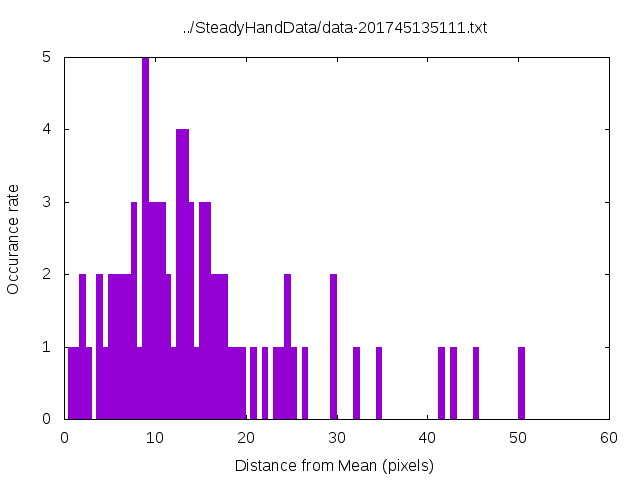
\includegraphics[scale=.5]{graph-data-201745135111.png} &
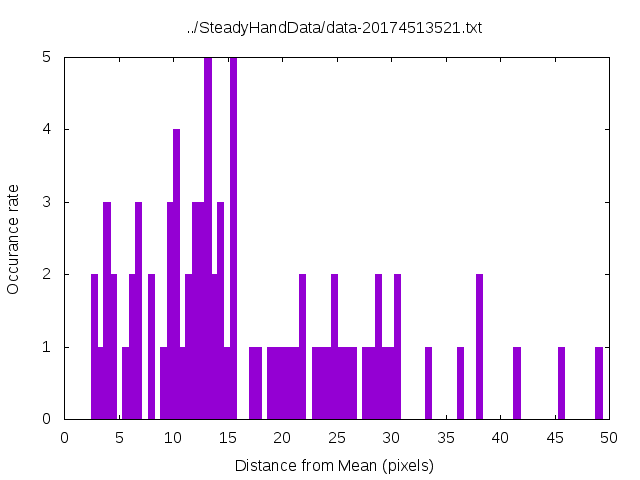
\includegraphics[scale=.5]{graph-data-20174513521.png}\\
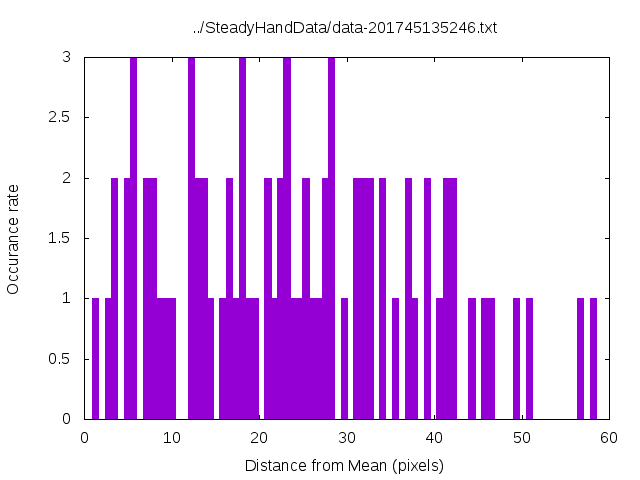
\includegraphics[scale=.5]{graph-data-201745135246.png} &
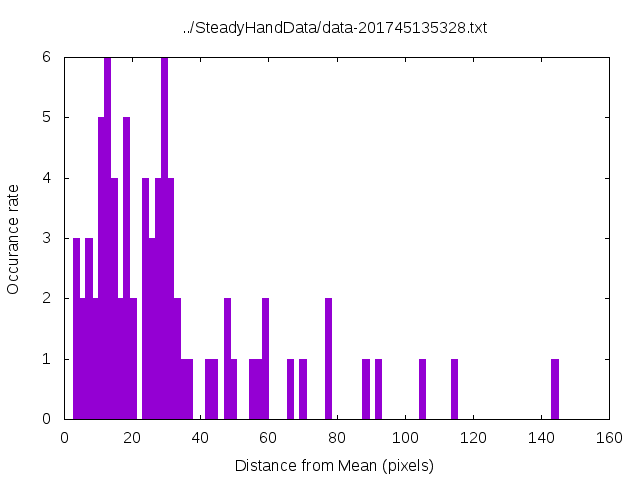
\includegraphics[scale=.5]{graph-data-201745135328.png}\\
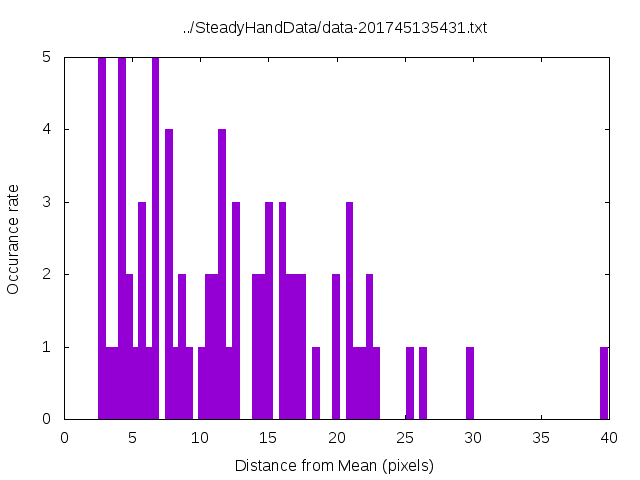
\includegraphics[scale=.5]{graph-data-201745135431.png} &
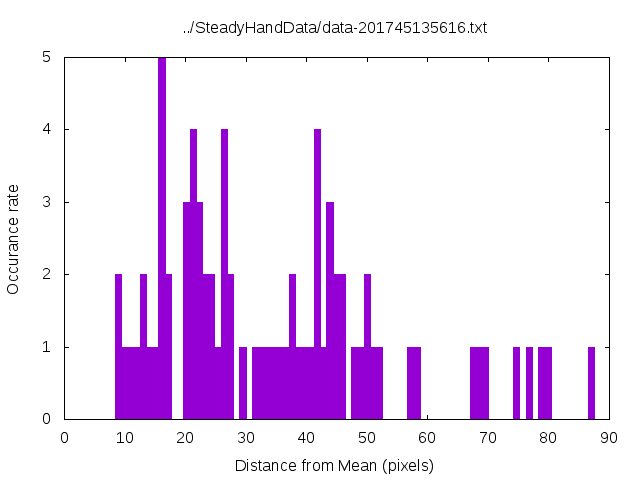
\includegraphics[scale=.5]{graph-data-201745135616.png}\\
\end{tabular}
\end{table}
\begin{table}
\begin{tabular}{cc}
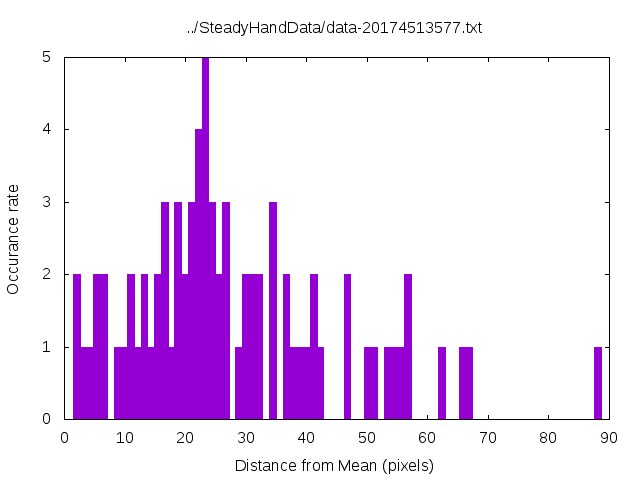
\includegraphics[scale=.5]{graph-data-20174513577.png} &
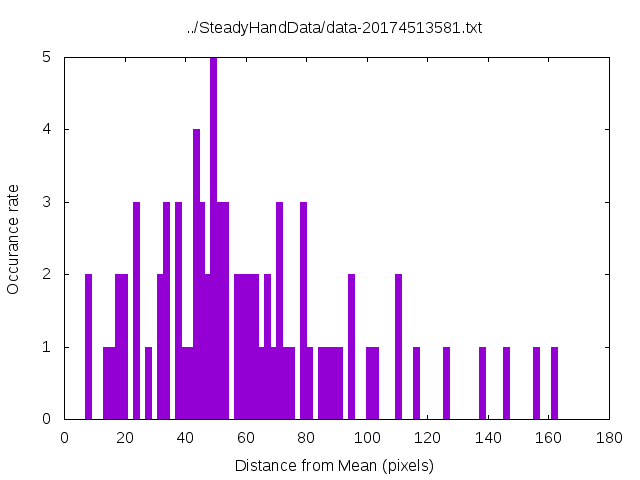
\includegraphics[scale=.5]{graph-data-20174513581.png}\\
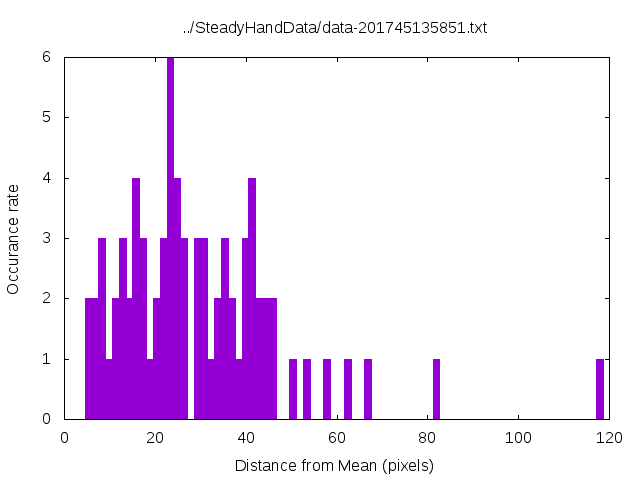
\includegraphics[scale=.5]{graph-data-201745135851.png} &
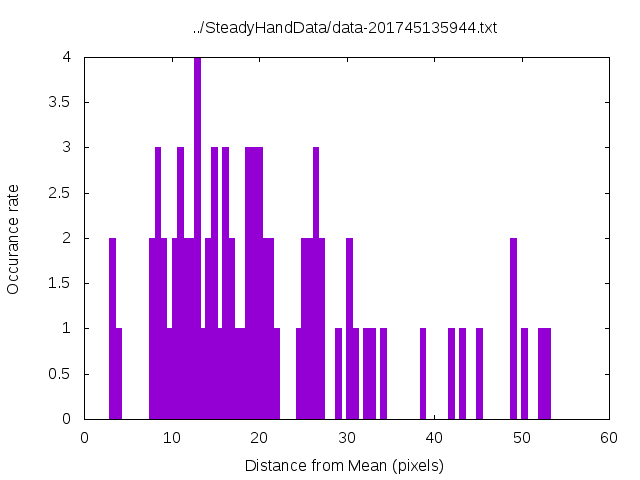
\includegraphics[scale=.5]{graph-data-201745135944.png}\\
\end{tabular}
\end{table}
\end{document}
